\documentclass[12pt]{ctexart}

%导包区###################################################################################
%\usepackage{mathrsfs}花体字母$\mathscr{A}$ 或者 $\mathcal{A}$
\usepackage{amssymb}
\usepackage{amsmath}
\usepackage{listings}
\usepackage{color}

\definecolor{dkgreen}{rgb}{0,0.6,0}
\definecolor{gray}{rgb}{0.5,0.5,0.5}
\definecolor{mauve}{rgb}{0.58,0,0.82}

\lstset{frame=tb,
	language=Python,
	aboveskip=3mm,
	belowskip=3mm,
	showstringspaces=false,
	columns=flexible,
	basicstyle={\small\ttfamily},
	numbers=none,
	numberstyle=\tiny\color{gray},
	keywordstyle=\color{blue},
	commentstyle=\color{dkgreen},
	stringstyle=\color{mauve},
	breaklines=true,
	breakatwhitespace=true,
	tabsize=3
}
\usepackage{colortbl,booktabs}%第二个包定义了几个*rule
\usepackage{enumerate}%编号
\usepackage{float}%图像浮动
\usepackage{enumitem} 
\usepackage{algorithm}  
\usepackage{algorithmicx}  
\usepackage{algpseudocode}  
\usepackage{amsmath}  %伪代码
\usepackage{ctex}
\usepackage{xeCJK}%中文字体
\usepackage[a4paper, top=2.54cm, bottom=2.54cm,left = 3.18cm, right = 3.18cm]{geometry}
%采用1.5倍行间距。中文小四号宋体,英文小四号Times New Roman
\setCJKmainfont{SimSun} %或\setCJKmainfont{KaiTi}
\setCJKmonofont{SimSun}
\setmainfont{Times New Roman}
\usepackage{setspace}%使用间距宏包
\usepackage{fontspec}%字体
\usepackage{fancyhdr}%页眉和页脚
\usepackage{graphicx}%插入图象
\usepackage{subfigure}%子图显示
\usepackage{ titletoc }%自定义目录
\usepackage[colorlinks,linkcolor=black]{hyperref}%目录链接,加上这个包生成目录自带连接
%绘图工具包
\usepackage{tikz,mathpazo}
\newcommand{\upcite}[1]{\textsuperscript{\textsuperscript{\cite{#1}}}}
\renewcommand{\sectionmark}[1]{\markboth{第\thesection 章\ #1}{}}
\usetikzlibrary{shapes.geometric, arrows}
\usetikzlibrary{calc}
% 流程图定义基本形状
%矩形
\tikzstyle{startstop} = [rectangle, rounded corners, minimum width = 1.5cm, minimum height=1cm,text centered, draw = black, fill = white!40]
\tikzstyle{input} = [rectangle, rounded corners, minimum width = 1.5cm, minimum height=1cm,text centered, draw = black, fill = gray!40]
\tikzstyle{output} = [rectangle, rounded corners, minimum width = 1.5cm, minimum height=1cm,text centered, draw = black, fill = gray!40]
%梯形
\tikzstyle{io} = [trapezium, trapezium left angle=70, trapezium right angle=110, minimum width=1cm, minimum height=1cm, text centered, draw=black, fill = blue!40]
%圆形
\tikzstyle{process} = [circle, minimum width=1cm, minimum height=1cm, text centered, draw=black, fill = white!50]
\tikzstyle{add} = [circle, minimum width=0.5cm, minimum height=0.5cm, text centered, draw=black, fill = white!50]
%菱形
\tikzstyle{decision} = [diamond, aspect = 3, text centered, draw=black, fill = green!30]
% 箭头形式
\tikzstyle{arrow} = [->,>=stealth]
\tikzstyle{line} =[thick,-, >= stealth]
\usepackage[justification=centering]{caption}
\usepackage{hyperref}%添加pdf属性
\hypersetup{
pdftitle={低分辨率下的文本定位识别研究与实现},
pdfauthor={陶光品1510742},
pdfsubject={本科生毕业论文}
}

%全局设置#################################################################################
%章节标题编号样式,字体间距
\CTEXsetup[name={第,章},number={\chinese{section}},format={\centering\heiti\zihao{3}}]{section}
\CTEXsetup[name={第,节},number={\chinese{subsection}},format={\centering\heiti\zihao{-3}}]{subsection}
\CTEXsetup[format={\raggedright\heiti\zihao{4}}]{subsubsection}
\newcommand{\RNum}[1]{\uppercase\expandafter{\romannumeral #1\relax}}%罗马数字
%文档开始#################################################################################
\begin{document}
	\begin{spacing}{1.5}%%行间距变为double-space
	\songti \zihao{3}
	\pagestyle{empty} % 封面没有页眉页脚
\begin{center} 
	\ \\
	\vspace{20pt}
	{\songti  \zihao{-0}{南\ 开\ 大\ 学}}\\
	\setlength{\baselineskip}{50pt}
	{\songti  \zihao{2}本\ 科\ 生\ 毕\ 业\ 论\ 文\ (设\ 计)}\\
\end{center} 
\vspace{50pt}
\qquad{\songti  \zihao{-3}中文题目:}\kaishu \zihao{-3} \textbf{\underline{低分辨率下的文本定位识别研究与实现\ \ \ \ }}

\ {\songti  \zihao{-3}外文题目:}\kaishu \zihao{-3}  \textbf{\underline{Scene Text Detection and Recognition Under}}

\qquad\qquad\quad\ \kaishu \zihao{-3} \textbf{\underline{Low Resolution \ \ \ \ \ \ \ \ \ \ \ \ \ \ \ \ \ \ \ \ \ \ \ \ \ \ \ \ \ \qquad\ \ \ }}\\
\setlength{\baselineskip}{25pt}\\
\vspace{40pt}
\begin{center}
	\begin{tabular}{l}
		\songti \zihao{4}学\qquad 号:\kaishu \zihao{4} \textbf{\underline{1510742\qquad\quad\ \ \ \ \ }}\\
		\songti \zihao{4}姓\qquad 名:\kaishu \zihao{4} \textbf{\underline{陶某某\ \ \ \ \ \ \ \ \ \ \ \ \ \ \ \ }}\\
		\songti \zihao{4}年\qquad 级:\kaishu \zihao{4} \textbf{\underline{2015级\quad\quad\quad\quad\ \ \ }}\\
		\songti \zihao{4}专\qquad 业:\kaishu \zihao{4} \textbf{\underline{计算机科学与技术}}\\
		\songti \zihao{4}系\qquad 别:\kaishu \zihao{4} \textbf{\underline{计算机科学与技术}}\\
		\songti \zihao{4}学\qquad 院:\kaishu \zihao{4} \textbf{\underline{计算机学院\quad\quad\quad}}\\
		\songti \zihao{4}指导教师:\kaishu \zihao{4} \textbf{\underline{王某\ \ 副教授\ \quad\quad}}\\
		\songti \zihao{4}完成日期:\kaishu \zihao{4} \textbf{\underline{2019年5月\quad\ \ \ \ \ }}\\

	\end{tabular}
\end{center}
\clearpage
\ \
\vspace{30pt}
\begin{center} \heiti \zihao{3}关于南开大学本科生毕业论文(设计)的声明
\end{center}
\songti \zihao{-4}

本人郑重声明:所呈交的学位论文,是本人在导师指导下进行研究工作所取得的研究成果。除文中已经注明引用的内容外,本学位论文的研究成果不包含任何他人创作的、已公开发表或者没有公开发表的作品的内容。对本论文所涉及的研究工作做出贡献的其他个人和集体,均已在文中以明确方式标明。本学位论文原创性声明的法律责任由本人承担。

\qquad\qquad\qquad\qquad\qquad 学位论文作者签名:\qquad\qquad 

\qquad\qquad\qquad\qquad\qquad\qquad\qquad\qquad\qquad\qquad 年\qquad 月\qquad 日

本人声明:该学位论文是本人指导学生完成的研究成果,已经审阅过论文的全部内容,并能够保证题目、关键词、摘要部分中英文内容的一致性和准确性。

\qquad\qquad\qquad\qquad 学位论文指导教师签名:\qquad\qquad 

\qquad\qquad\qquad\qquad\qquad\qquad\qquad\qquad\qquad\qquad 年\qquad 月\qquad 日
\clearpage
%中文摘要################################################################################
\fancyhf{}%清空当前设置
\setcounter{page}{1}
\pagestyle{fancy}
\pagenumbering{Roman}



\lhead{} \chead{摘要} \rhead{}
\lfoot{} \cfoot{\thepage} \rfoot{}
\renewcommand\headrulewidth{0.3pt}





\renewcommand{\abstractname}{\heiti \zihao{4} 摘\quad 要}
\titlecontents{section}
[0cm]%离左边界的距离
{\songti\zihao{3}}
{\contentslabel{4em}}%目录中第一章与引言的距离
{}%
{\titlerule*[0.5pc]{$\cdot$}\contentspage \hspace*{0cm}}%指引线格式
\begin{abstract}
	\addcontentsline{toc}{section}{摘要}
	\songti \zihao{-4}这是摘要部分。\\
	\ \\
	\heiti \zihao{-4}关键词:\songti \zihao{-4}换行与冒号对齐
\end{abstract}
\clearpage%另外起一页
\lhead{} \chead{Abstract} \rhead{}
\renewcommand{\abstractname}{\heiti \zihao{4} Abstract}
\begin{abstract}
	\addcontentsline{toc}{section}{Abstract}
	\setmainfont{Times New Roman}\zihao{-4}
	%\songti \zihao{4}
	This is abstract part.\\
	\ \\
	\qquad  \textbf{Key Words:}
\end{abstract}
\clearpage%另外起一页  
%以上指令中\chaptermark用于重新定义页眉内之章标题;
%其内容取自LaTeX的\markboth指令。事实上\markboth指令用于存放两项信息,分别
%存放于指令之后的两个大括号内。在book文件类别中,第一项为章名的相关信息;
%第二项为节标题的相关信息。故以上命令是重新定义章标题存放于页眉/页脚的内容,
%节标题不变,因此第二对大括号内为空白
%注:\markboth{leftmark}{rightmark} 在book文件类别下,\leftmark自动存录各章之章名,\rightmark记录节标题
%我们就可以用如下代码自动添加中文章节名了
%设置页眉页脚
\pagestyle{fancy}
\lhead{} \chead{\leftmark} \rhead{}
\lfoot{} \cfoot{\thepage} \rfoot{}
\renewcommand\headrulewidth{0.3pt}
\addcontentsline{toc}{section}{目录}
%目录区#########################################################################################
%重新设置正文目录
\titlecontents{section}[2.1cm]{\bfseries \zihao{-3} \vspace{5pt}}{\contentslabel{4em}}{\hspace*{-4em}}{~\titlerule*[0.6pc]{$.$}~\contentspage}

\titlecontents{subsection}[3.1cm]{\zihao{4}}{\contentslabel{4em}}{\hspace*{-2em}}{~\titlerule*[0.6pc]{$.$}~\contentspage}

\titlecontents{subsubsection}[4.1cm]{\zihao{-4}}{\contentslabel{4em}}{\hspace*{-2em}}{~\titlerule*[0.6pc]{$.$}~\contentspage}


\tableofcontents %—— 
\clearpage
%正文区##############################################################################
%\fancyhf{}%清空当前设置
\setcounter{page}{1}
\pagenumbering{arabic}
\section{绪论}
\zihao{-4}
每一章章节之间说明论文写作逻辑
\subsection{背景意义}
选题的背景意义。
\subsection{毕设内容}
新想法>算法复现>跑模型

可展示+工作量(代码量)

可读性强的论文,往往能从摘要看做了什么,从目录看怎么写的。
\clearpage
\section{相关工作}
论文一般从相关研究,实验方法,实验结果,总结展望几个方面展开,不过为了直观明显,建议不要按这种抽象的方式组织,替换成具体工作。
\subsection{节1}
\subsubsection{\zihao{4}子节1}子节内容。

\subsubsection{ \zihao{4}数学公式,上标引用,绘图示例}Laplacian pyramid\upcite{burt1983laplacian}第K层定义:$$L_{K}=G_{K}-UP(G_{K+1})\otimes filer\eqno(2.1)$$
公式按章标号,即章号.公式号。

绘图先定义结点样式和相对位置关系,然后画线或者箭头,也有丰富的样式可以选择。用 $\backslash$ref\{pyramid\}引用,括号里是图像的标签,在图像环境中声明,效果为:如图\ref{pyramid}所示:
\begin{figure}[htbp]
	\centering
	\begin{tikzpicture}[node distance=1.5cm]
	%定义流程图具体形状\node[样式](名称){标题};
	\node (DT) [startstop] {低通滤波器};
	\node (DS) [startstop,right of=DT,xshift=2cm] {下采样};
	\node (SC) [output,right of=DS,xshift=4cm,align=center] {输出N+1\\层图像(GP)};
	\node (US) [startstop,below of=DS,xshift=2cm,yshift=-0.2cm]{上采样};
	\node (CR) [startstop,below of=US,yshift=-0.2cm]{插值滤波器};
	\node(In)[input,below of=DT,yshift=-4cm]{N层输入图像};
	\node(CZ)[add,right of=In,xshift=4cm,align=center]{差值\\预测};
	\node(Out)[output,right of=CZ,xshift=2cm,align=center]{输出N层预\\测残差(LP)};
	\draw [arrow](DT) -- (DS);
	\draw [arrow](In) -- (DT);
	\draw [arrow](In) -- (CZ);
	\draw [arrow](CZ) -- (Out);
	\draw [arrow](DS) -- (SC);
	\draw [arrow](US) -- (CR);
	\draw [arrow](CR) -- (CZ);
	\draw [arrow]($(DS.east) + (1.22,0)$)-- (US);
	\end{tikzpicture}
	\caption{高斯金字塔(GP)和拉普拉斯金字塔(LP)的采样流程}  %图片的名称
	\label{pyramid}
\end{figure}
\subsection{文本检测识别性能评价方法}
\subsubsection{\zihao{4} 表格环境}一种更牛逼的方式是用表格工具生成表格,但我觉得表格工具有点麻烦,不直观,用excel制表截图插入更方便,不过这样caption显示的是图num:而不是表num:,建议还是用表格环境更好。
\begin{figure}[h]
	\centering
	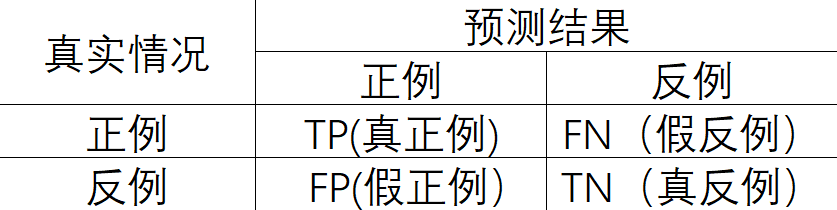
\includegraphics[width=0.6\textwidth]{figures/PR.PNG}
	\caption*{表1:分类混淆矩阵}
\end{figure} 
\subsubsection{\zihao{4} 项目编号使用}
\begin{itemize}
	\item[(1)]  编号括号、数字的样式都有具体格式,没仔细看
	\item[(2)] 项目2
	\item[(3)] 项目3
\end{itemize}
\subsubsection{\zihao{4} 算法伪代码}
用algorithm环境制作算法伪代码非常方便,基本的语法是输入输出,statement语句,函数块,控制语句等。基本实现效果如算法\ref{algorithm}。
\floatname{algorithm}{算法}  
\renewcommand{\algorithmicrequire}{\textbf{输入:}}  
\renewcommand{\algorithmicensure}{\textbf{输出:}}  
\begin{algorithm}[h]
	\caption{基于小波空间域的超分辨率算法} 
	\zihao{-4}
	\label{algorithm} 
	\begin{algorithmic}[1] %每行显示行号  
		\Require 低分辨率图像lr,超分辨率倍数Factor
		\Ensure 高分辨率图像hr 
		\Function {Super-resolution}{$lr,Factor$}  
		\State $hr_{t} \gets$ \Call{UpSampling}{$lr,Factor$}
		\State $hr_{g} \gets$ \Call{GaussianFilter}{$hr_{t}$}
		\For{(i=0;i<2;i++)} 
		\State $lr_{i} \gets$ \Call{DownSampling}{$hr_{g},Factor$}
		\State $ReconstructionError(i)=lr-lr_{i}$
		\State $Eh(i) \gets$ \Call{UpSampling}{$ReconstructionError(i)$}
		\State $hr(i+1)=Eh(i)+hr(i)$
		\EndFor 
		\State $hr \gets hr_{2}$
		\EndFunction
	\end{algorithmic}  
\end{algorithm} 
\clearpage
%除了新的一页,此外newpage也有相同功能,但clearpage更好用,可以保证图像的浮动。
关于tikz绘图包,可以像ps一样设置图层绘制更加复杂的图,不过用到的只有基本要素,下面再给一例:

\begin{figure}[htbp]
	\centering
	\begin{tikzpicture}[node distance=1.5cm]
	%\begin{pgfonlayer}{background}
	\node (IN) [input,align=center,x=1cm,y=1cm] {输入\\$I^{l}$};
	\node (FE1) [startstop, right of=IN,xshift=1cm,align=center] {3*3卷积};
	\node (FE2) [startstop, right of=FE1,xshift=1cm,align=center] {1*1卷积};
	\node (FE3) [startstop, right of=FE2,xshift=1cm,align=center] {上采样\\投影};
	\node (FE4) [startstop, right of=FE3,xshift=1cm,align=center] {下采样\\投影};
	
	\node (FE5) [startstop, below of=FE4,yshift=-1cm,align=center] {上采样\\投影};
	\node (FE6) [startstop, left of=FE5,xshift=-1cm,align=center] {下采样\\投影};
	\node (Concat) [startstop, left of=FE6,xshift=-1cm,align=center] {全连接};	
	\node (RC) [startstop, left of=Concat,xshift=-1cm,align=center] {3*3卷积};
	\node (OUT) [output,left of=RC,xshift=-1cm,align=center] {输出\\$I^{sr}$};
	\draw [arrow](IN) -- (FE1);
	\draw [arrow](FE1)-- (FE2);
	\draw [arrow](FE2)-- (FE3);
	\draw [arrow](FE3)--(FE4);
	\draw [arrow](FE5)--(FE6);
	\draw [arrow](FE4)node[xshift=1.5cm,yshift=-1cm] {多层稠密连接}  -- (FE5);
	\draw[->,dashed](FE3)--(FE6);
	\draw[arrow](FE6)--(Concat);
	\draw [arrow](Concat)--(RC);
	\draw [arrow](RC)--(OUT);
	\draw [dashed,thick](6.5,1)node[below left]{}--(11,1)node[below right]{};
	\draw [dashed,thick](6.5,1)node[below left]{}--(6.5,-3.5)node[below right]{};
	\draw [dashed,thick](11,1)node[below left]{}--(11,-3.5)node[below right]{};
	\draw [dashed,thick](6.5,-3.5)node[below left]{}--(11,-3.5)node[below right]{};
	%\end{pgfonlayer}
	\end{tikzpicture}
	\caption{DBPN网络结构}
	\label{extr}
\end{figure}
%\pgfdeclarelayer{background}
%\pgfsetlayers{main,background
%############################################################################################################
\clearpage
\section{实验结果}
论文写作逻辑。
\subsection{数据集}
数据集多多益善,也可以作为展望中的一部分。
\subsection{自动评测}
在数据处理时。可以写一个自动评测python脚本来进行数据分析,例如用python os包(文件目录访问读写以及代码中cmd指令的执行),skimage包(提供丰富图像操作以及计算图像评价指标),CSV和Pandas包(保存分析处理评价指标,数值分析),matplotlib包绘制结果对比图,实现的自动评测脚本过程如图\ref{auto}:
\begin{figure}[htbp]
	\centering
	\begin{tikzpicture}[node distance=1.5cm]
	%定义流程图具体形状\node[样式](名称){标题};
	\node (GT) [input,align=center,x=0.5cm,y=0.5cm] {输入真值\\数据集};
	\node (LR) [startstop,align=center, right of=GT,xshift=2cm] {得到低分辨率\\有序数据集};
	\node (SR) [startstop,align=center, right of=LR,xshift=3cm] {命令行执行\\各超分辨率算法};
	\node (QL) [startstop, align=center,right of=SR,xshift=2cm] {计算图像\\评价指标};
	\node (CSV) [startstop,align=center, below of=QL,yshift=-1cm] {保存\\CSV文件};
	\node (ANA) [startstop,align=center, left of=CSV,xshift=-2cm] {数据\\分析};
	\node(PLOT) [output,align=center, left of=ANA,xshift=-2cm] {绘制指标\\对比图};
	\draw [arrow](GT) -- (LR);
	\draw [arrow](LR)-- (SR);
	\draw [arrow](SR)-- (QL);
	\draw [arrow](QL)--(CSV);
	\draw [arrow](CSV)--(ANA);
	\draw [arrow](ANA)--(PLOT);
	\end{tikzpicture}
	\caption{自动评测流程}
	\label{auto}
\end{figure}
在得到CSV文件后可以直接用office Excel进行数据分析,通过自动评测可以减少重复输入测试,大大减少模型运行,数据测得,结果分析的时间,提高工作效率。
\clearpage
\subsection{图像展示}
\begin{figure}[h]
	\centering
	\begin{minipage}[t]{0.3\linewidth}
		
\includegraphics[width=1\textwidth]{figures/1.jpg}
		\caption*{吃萝卜的龙猫}
	\end{minipage} 
	\hfill
	\begin{minipage}[t]{0.3\linewidth}
		
\includegraphics[width=1\textwidth]{figures/2.jpg}
		\caption*{\protect 头上有老\\鼠的龙猫}
	\end{minipage}
	\hfill
	\begin{minipage}[t]{0.3\linewidth}
		
\includegraphics[width=1\textwidth]{figures/3.jpg}
		\caption*{吃西瓜的龙猫}
	\end{minipage} 
	\begin{minipage}[t]{0.3\linewidth}
		
\includegraphics[width=1\textwidth]{figures/4.jpg}
		\caption*{雄性龙猫}
	\end{minipage}
	\hfill
	\begin{minipage}[t]{0.3\linewidth}
		
\includegraphics[width=1\textwidth]{figures/5.jpg}
		\caption*{雌性龙猫}
	\end{minipage}
	\hfill
	\begin{minipage}[t]{0.3\linewidth}
		
\includegraphics[width=1\textwidth]{figures/6.jpg}
		\caption*{大龙猫}
	\end{minipage}
	\caption{各种龙猫}
	\label{2x}
\end{figure}
\clearpage
\section{总结和展望}
总结论文得到的结论成果,存在的问题和可能的解决办法。
\clearpage%另外起一页
%往目录里面添加参考文献索引
\addcontentsline{toc}{section}{参考文献}
%bibtex文献应用
\bibliographystyle{IEEEtran}
\bibliography{bs}
%手动文献
%	\begin{thebibliography}{1}
%		\bibitem{liu} 刘海洋. \LaTeX 入门 [M]. 北京: 电子工业出版社, 2013.
%		\bibitem{hu}  胡伟. \LaTeX 2e完全学习手册(第二版). 北京: 清华大学出版社, 2013.
%	\end{thebibliography}
\clearpage%另外起一页
\fancyhf{}%清空当前设置
\thispagestyle{fancy}
\lhead{} \chead{致谢} \rhead{}
\lfoot{} \cfoot{\thepage} \rfoot{}
\renewcommand\headrulewidth{0.3pt}
\addcontentsline{toc}{section}{致谢}
\begin{center}
	\heiti \zihao{4} 致谢
\end{center}
这里是致谢部分:

毕设是学习的过程,感谢这次毕设机,让我看到了自己的不足,同时也让我学到了很多东西。
\end{spacing}
\newpage
\fancyhf{}%清空当前设置
\pagestyle{fancy}
\lhead{} \chead{附录A} \rhead{}
\lfoot{} \cfoot{\thepage} \rfoot{}

\addcontentsline{toc}{section}{附录A}
\titlecontents{subsection}[2.1cm]{\zihao{4}}{\contentslabel{4em}}{\hspace*{-2em}}{~\titlerule*[0.6pc]{$.$}~\contentspage}
附上代码体现代码工作量
\addcontentsline{toc}{subsection}{A.1 XXX的实现}
xxx的实现如下(c++ opencv):
\lstset{frame=tb,
	language=c++,
	aboveskip=3mm,
	belowskip=3mm,
	showstringspaces=false,
	columns=flexible,
	basicstyle={\small\ttfamily},
	numbers=none,
	numberstyle=\tiny\color{gray},
	keywordstyle=\color{blue},
	commentstyle=\color{dkgreen},
	stringstyle=\color{mauve},
	breaklines=true,
	breakatwhitespace=true,
	tabsize=3
}
\begin{lstlisting}
#include <iostream>
	cout<<"helloworld"<<endl;
	return 0;
}
\end{lstlisting}
\lstset{frame=tb,
	language=python,
	aboveskip=3mm,
	belowskip=3mm,
	showstringspaces=false,
	columns=flexible,
	basicstyle={\small\ttfamily},
	numbers=none,
	numberstyle=\tiny\color{gray},
	keywordstyle=\color{blue},
	commentstyle=\color{dkgreen},
	stringstyle=\color{mauve},
	breaklines=true,
	breakatwhitespace=true,
	tabsize=3
}
\addcontentsline{toc}{subsection}{A.2 自动评测实现}
评测部分主要函数简要实现如下(python):
\begin{lstlisting}
#调用时使用process(gtpath,'wsd','raisr',……)
def process(gtpath,*args):
#对真值图像进行下采样和重编号命名:
	paths = glob.glob(gtpath+'/*.jpg')
	paths.sort()
	for file in paths:
	(filepath, tempfilename) = os.path.split(file)
	(filename, extension) = os.path.splitext(tempfilename)
	img = cv2.imread(file, 1)  
	factor=2
	size = (int(img.shape[1]/factor),int(img.shape[0]/factor))  
	shrink = cv2.resize(img, size, interpolation=cv2.INTER_LINEAR)
	cv2.imwrite("LR/"+filename+".jpg",shrink)
	for i in range(len(args)):
#cmd执行python脚本
		os.popen('python ' + args[i]+'/'+args[i] + '.py')
#评测对比PSNR,输入为真值路径以及图像数量,SSIM方法类似
def evalpsnr(gtpath, num):
	out = open('psnr.csv', 'w', newline='')
	csv_write = csv.writer(out, dialect='excel')
	csv_write.writerow(['IMG#', 'WSD', 'RAISR','SRGAN','DBPN'])
	gt = skimage.io.imread(gtpath + '/' + str(j) + '.jpg')
	for j in range(num):
		wsd_img = skimage.io.imread('wsd_result'+str(j) + '.jpg')
		wsd_psnr = skimage.measure.compare_psnr(gt, wsd_img)
		#ssim = skimage.measure.compare_ssim(gt, test, multichannel=True)
		(……计算其他方法method_psnr)
		csv_write.writerow([j, wsd_psnr,raisr_psnr,srgan_psnr,dbpn_pnsr])
	out.close()
#使用pandas库对CSV求最大值,最小值,平均值等聚合统计
def analyse(path):
	df = pandas.read_csv(path+"/psnr.csv")
	print(df)
#求某一方法处理后下psnr最佳和最差对应图像编号和psnr均值
	print(df['WSD'].idxmin(),df['WSD'].idxmax(),df['WSD'].mean())
#matplotlib.plot绘制psnr对比折线图,横坐标为图像编号,纵坐标为PSNR
#不同方法标注不同颜色
	x = np.linspace(1, num, num)
	print(x)
	l1 = plt.plot(x, df['WSD'], 'blue')
	l2 = plt.plot(x, df['RAISR'],'purple')
	l3 = plt.plot(x, df['SRGAN'], 'green')
	l2 = plt.plot(x, df['DBPN'],'yellow')
	plt.title('PSNR')
	plt.xlabel('IMAGE')
	plt.ylabel('PSNR')
	plt.legend((l1[0], l2[0],l3[0],l4[0]), ('WSD', 'RAISR','SRGAN','DBPN'))
	plt.show()
\end{lstlisting}
\end{document}